\section{Introduction}

Having developed an understanding of how the parameters of a deep network effect the underlying geometry of the deep network, we can start investigating the precise effects of operators on the functional geometry of a deep network and how this translates into properties of the deep network. Specifically, we focus on the normalisation operations and how they initialise and regularise deep networks.

\section{Batch Normalisation}\label{sec:batch_norm}

For a batch normalised layer, let $$\left[\mathbf{h}^{(\ell)}\right]_i=\frac{\left\langle\left[W^{(\ell)}\right]_{i,\cdot},\mathbf{z}^{(\ell-1)}\right\rangle-\left[\mu^{(\ell)}\right]_i}{\left[\sigma^{(\ell)}\right]_i},$$so that $\mathbf{h}^{(\ell)}$ is the pre-activation\footnote{This is well-defined provided $\left\Vert\left[W^{(\ell)}\right]_{i,\cdot}\right\Vert_2^2>0$ and the inputs of the batch are not orthogonal to $\left[W^{(\ell)}\right]_{i,\cdot}$.} of layer $\ell$ and $\mathbf{z}^{(\ell)}=\sigma_{\text{act}}\left(\mathbf{h}^{(\ell)}\right)$.

The separation of regimes induced by the affine components of $\sigma_{\text{act}}$\footnote{In this analysis we are assuming that $\sigma_{\text{act}}$ consists of two affined components joining at the origin.} is governed by the hyperplane arrangement $$\partial\Omega^{(\ell)}=\bigcup_{i=1}^{d^{(\ell)}}\mathcal{H}^{(\ell)}_i$$where $$\mathcal{H}^{(\ell)}_i=\left\{\mathbf{z}^{(\ell-1)}\in\mathbb{R}^{d^{(\ell-1)}}:\left[\mathbf{h}^{(\ell)}\right]_i=0\right\}$$is a $d^{(\ell)}$-dimensional hyperplane.\footnote{Note that $\mathcal{H}^{(\ell)}_i$ is independent of $\left[\sigma^{(\ell)}\right]_i$.}

\subsection{Single Layer Analysis}\label{subsec:single_layer_analysis}

\begin{lemma}\label{lem:distance_to_hyperplane}
    The Euclidean distance from a point $\mathbf{v}$ in layer $\ell$'s input space and $\mathcal{H}^{(\ell)}_i$ is $$d\left(\mathbf{v},\mathcal{H}^{(\ell)}_i\right)=\frac{\left\vert\left\langle\left[W^{(\ell)}\right]_{i,\cdot},\mathbf{v}\right\rangle-\left[\mu^{(\ell)}\right]_i\right\vert}{\left\Vert\left[W^{(\ell)}\right]_{i,\cdot}\right\Vert_2},$$when $\left\Vert\left[W^{(\ell)}\right]_{i,\cdot}\right\Vert_2>0$.\footnote{For a proof refer to \citet{alexanderschrijverTheoryLinearInteger1998}.}
\end{lemma}

Let $\mathcal{V}$ be a collection of points in $\ell$'s input space. From Lemma \ref{lem:distance_to_hyperplane}, it follows that the unit least squares distance is 
\begin{equation}\label{eq:unit_least_squares}
    \mathcal{L}_i\left(\left[\mu^{(\ell)}\right]_i;\mathcal{V}\right)=\frac{1}{\vert\mathcal{V}\vert}\sum_{\mathbf{v}\in\mathcal{V}}d\left(\mathbf{v},\mathcal{H}^{(\ell)}_i\right)^2:=\frac{\left[\sigma^{(\ell)}\right]_{\ell,i}}{\left\Vert\left[W^{(\ell)}\right]_{i,\cdot}\right\Vert_2^2}
\end{equation}
for $i=1,\dots,d^{(\ell)}$ where the total least squares distance is $$\mathcal{L}\left(\mu^{(\ell)};\mathcal{V}\right)=\sum_{i=1}^{d^{(\ell)}}\mathcal{L}_i\left(\left[\mu^{(\ell)}\right]_i;\mathcal{V}\right).$$

\begin{theorem}\label{thm:minimising_tls}
    Consider a deep network layer $\ell$ equipped with batch normalisation. Let $\mathcal{B}^{(\ell)}\subseteq\mathcal{X}^{(\ell)}$ be a mini-batch. Then $\mu^{(\ell)}$ as given by \eqref{eq:bn_parameters} is the unique minimiser of $\mathcal{L}\left(\mu^{(\ell)};\mathcal{B}^{(\ell)}\right)$.
\end{theorem}

\begin{tproof}
    Consider the optimisation problem $$\min_{\mu\in\mathbb{R}^{d^{(\ell)}}}\mathcal{L}\left(\mu;\mathcal{Z}\right).$$Since the problem is unconstrained and the sum is separable, we can focus on $[\mu]_i$, yielding the optimisation problem $$\min_{[\mu]_i\in\mathbb{R}}\sum_{\mathbf{z}\in\mathcal{Z}}\frac{\left\vert\left\langle\left[W^{(\ell)}\right]_{i,\cdot},\mathbf{z}\right\rangle-[\mu]_i\right\vert^2}{\left\Vert\left[W^{(\ell)}\right]_{i,\cdot}\right\Vert_2^2}.$$Observe that, 
    \begin{align*}
        \partial\left(\sum_{\mathbf{z}\in\mathcal{Z}}\frac{\left\vert\left\langle\left[W^{(\ell)}\right]_{i,\cdot},\mathbf{z}\right\rangle-[\mu]_i\right\vert^2}{\left\Vert\left[W^{(\ell)}\right]_{i,\cdot}\right\Vert_2^2}\right)&=-2\sum_{\mathbf{z}\in\mathcal{Z}}\frac{\left\langle\left[W^{(\ell)}\right]_{i,\cdot},\mathbf{z}\right\rangle}{\left\Vert\left[W^{(\ell)}\right]_{i,\cdot}\right\Vert_2^2}\\&\quad+2\vert\mathcal{Z}\vert\frac{[\mu]_i}{\left\Vert\left[W^{(\ell)}\right]_{i,\cdot}\right\Vert_2^2}.
    \end{align*}
    It follows that the first derivative is zero if and only if $$[\mu]_i=\frac{1}{\vert\mathcal{Z}\vert}\sum_{\mathbf{z}\in\mathcal{Z}}\left\langle\left[W^{(\ell)}\right]_{i,\cdot},\mathbf{z}\right\rangle.$$Second derivative calculations confirm that this turning point is a minimum. By aggregating these across each of the $d^{(\ell)}$ dimensions, we deduce the desired result.
\end{tproof}

\begin{remark}
    For concreteness we note that by taking $\mathcal{B}^{(\ell)}=\mathcal{X}^{(\ell)}$ in Theorem \ref{thm:minimising_tls} we deduce that $\bar{\mu}^{(\ell)}$ is the unique minimiser of $\mathcal{L}\left(\mu^{(\ell)};\mathcal{X}^{(\ell)}\right)$.
\end{remark}

\begin{definition}
    A collection of hyperplanes $\mathcal{H}$ is central if $$\bigcap_{H\in\mathcal{H}}H\neq\emptyset.$$
\end{definition}

\begin{corollary}
    On $\mathcal{Z}\subseteq\mathcal{X}$, the induced arrangement of hyperplanes $\partial\Omega^{(\ell)}$ is central.
\end{corollary}

\begin{tproof}
    Let $\bar{\mathbf{z}}$ be the centroid of $\mathcal{Z}$. For $i\in\left\{1,\dots,d^{(\ell)}\right\}$ observe that
    \begin{align*}
        \left\langle\left[W^{(\ell)}\right]_{i,\cdot},\bar{\mathbf{z}}\right\rangle&=\left\langle\left[W^{(\ell)}\right]_{i,\cdot},\frac{1}{\vert\mathcal{Z}\vert}\sum_{\mathbf{z}\in\mathcal{Z}}\mathbf{z}\right\rangle\\&=\frac{1}{\vert\mathcal{Z}\vert}\sum_{\mathbf{z}\in\mathcal{Z}}\left\langle\left[W^{(\ell)}\right]_{i,\cdot},\mathbf{z}\right\rangle\\&\overset{\eqref{eq:bn_parameters}}{=}\left[\mu^{(\ell)}\right]_i.
    \end{align*}
    Therefore, $\bar{\mathbf{z}}\in\mathcal{H}^{(\ell)}_i$. Since, $i$ was arbitrary it follows that $$\bar{\mathbf{z}}\in\bigcap_{i=1}^{d^{(\ell)}}\mathcal{H}^{(\ell)}_i,$$meaning the arrangement $\partial\Omega^{(\ell)}$ is central.
\end{tproof}

In this analysis, we see that $\mu^{(\ell)}$ has a direct influence on the partitioning of a deep network layer's input space. The effect of the parameter $\sigma^{(\ell)}$ are introduced when composing deep network layers.

\subsection{Multilayer Analysis}

Similarly to Section \ref{subsec:single_layer_analysis}, we have $$\partial\Omega^{(1,\dots,\ell)}=\bigcup_{j=1}^{\ell}\bigcup_{i=1}^{d^{(j)}}\left\{\mathbf{x}\in\mathbb{R}^{d^{(1)}}:\left[\mathbf{h}^{(j)}\right]_i=0\right\}=:\bigcup_{j=1}^{\ell}\bigcup_{i=1}^{d^{(j)}}\mathcal{F}^{(j)}_{i,\omega}.$$In this scenario, the hyperplanes $\mathcal{H}^{(j)}_i$ are folded through the preceding layers to form facets $$\mathcal{F}^{(j)}_{i,\omega}=\left\{\mathbf{x}\in\omega:\left[\mathbf{h}^{(j)}\right]_i=0\right\}$$for $\omega\in\Omega^{(1,\dots,j)}$.\footnote{We can characterise the facets using the regions of $\Omega^{(1,\dots,j)}$, since the folds only happen at the boundaries of these regions as within the regions the transformation is affine.}With $\mathcal{F}^{(j)}_{i}:=\bigcup_{\omega\in\Omega^{(1,\dots,j)}}\mathcal{F}^{(j)}_{i,\omega}$ we can write $$\partial\Omega^{(1,\dots,\ell)}=\bigcup_{j=1}^{\ell}\bigcup_{i=1}^{d^{(j)}}\mathcal{F}^{(j)}_{i}.$$

\paragraph{The Effect of $\mu^{(\ell)}$.}

\begin{theorem}\label{thm:effect_mean_bn_multilayer}
    Consider a deep network layer $\ell>1$ equipped with batch normalisation. Suppose that layers $1,\dots,\ell-1$ have fixed batch normalisation parameters. Let $\mu^{(\ell)}$ and $\tilde{\mu}^{(\ell)}$ yield hyperplanes $\mathcal{H}^{(\ell)}_i$ and $\tilde{\mathcal{H}}^{(\ell)}_i$ which are folded into $\mathcal{F}^{(\ell)}_i$ and $\tilde{\mathcal{F}}^{(\ell)}_i$ respectively. Then, $d\left(\mathbf{z}^{(\ell)}(\mathbf{x}),\mathcal{H}^{(\ell)}_i\right)<d\left(\mathbf{z}^{(\ell)}(\mathbf{x}),\tilde{\mathcal{H}}^{(\ell)}_i\right)$ implies that $d\left(\mathbf{x},\mathcal{F}^{(\ell)}_i\right)<d\left(\mathbf{x},\tilde{\mathcal{F}}^{(\ell)}_i\right)$.\footnote{Here, $d\left(\mathbf{x},\mathcal{F}^{(\ell)}_{i}\right)=\min_{\mathbf{x}^\prime\in\mathcal{F}^{(\ell)}_{i}}\left\Vert\mathbf{x}-\mathbf{x}^\prime\right\Vert^2$.}
\end{theorem}

\begin{tproof}
    Let $$\mathbf{x}^*=\argmin_{\mathbf{u}\in\mathcal{F}_{\ell,i}}\left\Vert\mathbf{x}-\mathbf{u}\right\Vert_2.$$Let $l:[0,1]\to\mathbb{R}^d$ be given by $$l(\theta)=\mathbf{x}^*\theta+(1-\theta)\mathbf{x}.$$In the input space of layer $\ell$, the line $l$ becomes the piecewise affine parametric line $$\mathbf{z}^{(\ell-1)}(\theta)=\left(f_{\ell-1}\circ\dots\circ f_1\right)(l(\theta)).$$Now if there exists $\theta^\prime<1$ such that $\mathbf{z}^{(\ell-1)}\left(\theta^\prime\right)\in\mathcal{H}^{(\ell)}_i$ then there exists $\theta<1$ such that $l(\theta)\in\mathcal{F}^{(\ell)}_i$, Figure \ref{fig:multilayer_analysis_batchnorm_proof}.
    \begin{figure}
        \centering
        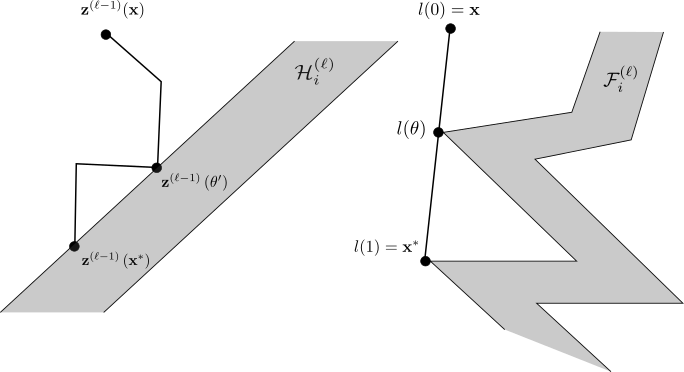
\includegraphics[width=0.75\linewidth]{drawings/multilayer_analysis_batchnorm_proof.png}
        \caption{}
        \label{fig:multilayer_analysis_batchnorm_proof}
    \end{figure}
    In other words, if the hyperplane $\mathcal{H}^{(\ell)}_i$ is bought closer to $\mathbf{z}^{(\ell-1)}(\mathbf{x})$ within the input space of layer $\ell$, then $\mathcal{F}^{(\ell)}_i$ is bought closer to $\mathbf{x}$. 
\end{tproof}

That is, translating hyperplanes closer to $\mathbf{z}^{(\ell)}$ in the input space of layer $\ell$, moves the folded hyperplane closer to $\mathbf{x}$ in the input space of the deep network.

\begin{corollary}
    Consider the setting of Theorem \ref{thm:effect_mean_bn_multilayer}. Then $\mathbf{z}^{(\ell)}(\mathbf{x})$ lies on the hyperplane $\mathcal{H}^{(\ell)}_i$ for some $i$ if and only if $\mathbf{x}$ lies on the corresponding folder hyperplane $\mathcal{F}^{(\ell)}_i$ in the input space of the deep network.
\end{corollary}

\paragraph{The Effect of $\sigma^{(\ell)}$.}

The parameter $\sigma^{(\ell)}$ optimises the dihedral angles between adjacent facets of the folded hyperplanes, to direct them toward the training data. For an input $\mathbf{z}$, let $Q^{(\ell)}$ be the square diagonal matrix with entries $$\left[Q^{(\ell)}\right]_{i,i}=\begin{cases}\frac{\alpha}{\left[\sigma^{(\ell)}\right]_i}&\left[\mathbf{h}^{(\ell)}\right]_i<0\\\frac{1}{\left[\sigma^{(\ell)}\right]_i}&\left[\mathbf{h}^{(\ell)}\right]_i\geq0,\end{cases}$$where $\mathbf{h}^{(\ell)}$ is the pre-activation of $\mathbf{z}$, and $\alpha$ is a parameter dependent on the activation function operating on layer $\ell$.\footnote{For ReLU we set $\alpha=0$, for leaky ReLU we set $\alpha=-1$, for absolute value we set $\alpha=-1$.}

The matrix $Q^{(\ell)}$ is constant across each region $\omega\in\Omega^{(\ell)}$. We will note this dependency with $Q^{(\ell)}(\omega)$.

\begin{theorem}\label{thm:effect_std_bn_multilayer}
    Consider a two-layer batch normalised equipped deep network employing a leaky-ReLU or absolute value activation function. Let $\omega,\omega^\prime\in\Omega$ be adjacent regions whose boundaries contain the facets $\mathcal{F}_{2,i,\omega}$ and $\mathcal{F}_{2,i,\omega^\prime}$, which are created from folding across the shared hyperplane boundary $\mathcal{H}^{(1)}_i$. The dihedral angles between these hyperplanes are $$\begin{cases}\theta\left(\mathcal{F}^{(2)}_{i,\omega},\mathcal{H}^{(1)}_j\right)=\arccos\left(\frac{\left\vert\left[W^{(2)}\right]_{i,\cdot}^\top Q^{(1)}(\omega)W^{(1)}\left[W^{(1)}\right]_{j,\cdot}\right\vert}{\left\Vert\left[W^{(2)}\right]_{i,\cdot}^\top Q^{(1)}(\omega)W^{(1)}\right\Vert\left\Vert\left[W^{(1)}\right]_{j,\cdot}\right\Vert}\right)\\\theta\left(\mathcal{F}^{(2)}_{i,\omega^\prime},\mathcal{H}^{(1)}_j\right)=\arccos\left(\frac{\left\vert\left[W^{(2)}\right]_{i,\cdot}^\top Q^{(1)}(\omega^\prime)W^{(1)}\left[W^{(1)}\right]_{j,\cdot}\right\vert}{\left\Vert\left[W^{(2)}\right]_{i,\cdot}^\top Q^{(1)}\left(\omega^\prime\right)W^{(1)}\right\Vert\left\Vert\left[W^{(1)}\right]_{j,\cdot}\right\Vert}\right)\\\theta\left(\mathcal{F}^{(2)}_{i,\omega},\mathcal{F}^{(2)}_{i,\omega^\prime}\right)=\arccos\left(\frac{\left\vert\left[W^{(2)}\right]_{i,\cdot}^\top Q^{(1)}(\omega)W^{(1)}\left(W^{(1)}\right)^\top Q^{(1)}\left(\omega^\prime\right)\left[W^{(2)}\right]_{i,\cdot}\right\vert}{\left\Vert\left[W^{(2)}\right]_{i,\cdot}^\top Q^{(1)}(\omega)W^{(1)}\right\Vert\left\Vert\left[W^{(2)}\right]_{i,\cdot}^\top Q^{(1)}\left(\omega^\prime\right)W^{(1)}\right\Vert}\right).\end{cases}$$
\end{theorem}

\begin{remark}
    Note that $Q^{(1)}(\omega)$ and $Q^{(1)}\left(\omega^\prime\right)$ differ only in the $(i,i)$ entry where one takes the value $\frac{1}{\left[\sigma^{(1)}\right]}$ and the other $\frac{\alpha}{\left[\sigma^{(1)}\right]}$. Furthermore, recall that from \eqref{eq:unit_least_squares} we have $\left[\sigma^{(\ell)}\right]_i^2\propto\min_{\mu^{(\ell)},i}\mathcal{L}\left(\left[\mu^{(\ell)}\right]_i;\mathcal{B}^{(\ell)}\right)$. Therefore, using Theorem \ref{thm:effect_std_bn_multilayer} we yield the following insights.
    \begin{itemize}
        \item If $\mathcal{H}^{(1)}_i$ is well-aligned with the training data $\mathcal{B}^{(1)}$, then the total least squares error, and hence $\left[\sigma^{(1)}\right]_i^2$, will be small. For the absolute value activation function it follows that $\theta\left(\mathcal{F}^{(2)}_{i,\omega},\mathcal{H}^{(1)}_i\right)\approx0$ and $\theta\left(\mathcal{F}^{(2)}_{i,\omega^\prime},\mathcal{H}^{(1)}_i\right)\approx0$, meaning $\mathcal{F}^{(2)}_{i,\omega}$ and $\mathcal{F}^{(2)}_{i,\omega^\prime}$ are folded to closely align with $\mathcal{H}^{(1)}_i$ and thus the data.
        \item If $\mathcal{H}^{(1)}_i$ is not well-aligned with the training data $\mathcal{B}^{(1)}$, then the total least squares error, and hence $\left[\sigma^{(1)}\right]_i^2$, will be large. Forcing $Q^{(1)}(\omega)\approx Q^{(1)}\left(\omega^\prime\right)$, making $\theta\left(\mathcal{F}^{(2)}_{i,\omega},\mathcal{F}^{(2)}_{i,\omega^\prime}\right)\approx\pi$, meaning that $\mathcal{H}^{(1)}_i$ will not appreciably fold intersection the layer two facets.
    \end{itemize}
\end{remark}

\subsection{Initialization Scheme}

In the case of binary classification, we can concretely intuit on the effect of batch normalisation.

\begin{proposition}\label{prop:initialisation_bn_binary_classification}
    Consider a $L$-layer deep network configured as a binary classifier on training data $\mathcal{X}$ using a leaky ReLU activation function at each layer, arbitrary weights $W^{(\ell)}$ at each layer, batch normalisation at layers $\ell=1,\dots,L-1$, and layer $L$ an affine layer with zero bias. Then for any training mini-batch from $\mathcal{X}$, there will be at least one data point on either side of the decision boundary.
\end{proposition}

\begin{tproof}
    Each mini-batch input to the last layer will have one input whose entries contain positive and negative values. Hence each dimension will have at least one negative value with the other being positive, or vice-versa. Since the last layer has zero bias, the decision boundary is the hyperplanes of zero level sets of each output unit. Since being on one side of the decision boundary in the deep network's input space is equivalent to being on one side of the linear decision boundary in the last layer's input space, there has to be at least one sample on one side of the decision boundary compared to the other samples.
\end{tproof}

In the setting of Proposition \ref{prop:initialisation_bn_binary_classification}, batch normalisation primes learning through stochastic gradient descent by ensuring the decision boundary passes through every mini-batch.

\subsection{Jitter}

The parameters $\mu^{(\ell)}$ and $\sigma^{(\ell)}$ can be thought of as stochastic estimators to $\bar{\mu}^{(\ell)}$ and $\bar{\sigma}^{(\ell)}$ respectively.

\begin{proposition}\label{prop:jitter_bn}
    Consider layer $\ell>1$ of a batch normalised deep network. Assume that inputs $\mathbf{z}^{(\ell-1)}$ are independent and identically distributed, with the distribution having zero mean and covariance matrix $\mathrm{diag}(\mathbf{m}\rho)$. Then $$\mathrm{var}\left(\left[\mu^{(\ell)}\right]_i\right)=\frac{\left\langle\left[W^{(\ell)}\right]_{i,\cdot}^2,\mathbf{m}\rho\right\rangle}{\left\vert\mathcal{B}^{(\ell)}\right\vert}$$and$$\mathrm{var}\left(\left[\sigma^{(\ell)}\right]_i^2\right)=\frac{1}{\left\vert\mathcal{B}^{(\ell)}\right\vert}\left(\left[\phi^{(\ell)}\right]_i-\frac{\left\langle\left[W^{(\ell)}\right]_i^2,\mathbf{m}\rho\right\rangle\left(\left\vert\mathcal{B}^{(\ell)}\right\vert-3\right)}{\left\vert\mathcal{B}^{(\ell)}\right\vert-1}\right),$$where $\left[W^{(\ell)}\right]_i^2$ is coordinate-wise and $\left[\phi^{(\ell)}\right]_i$ is the fourth-order central moment of $\left\langle\left[W^{(\ell)}\right]_i,\mathbf{z}^{(\ell)}\right\rangle$.
\end{proposition}

Proposition \ref{prop:jitter_bn} formalises the intuition that batch normalisation introduces noise into the learning process. 

\section{Layer Normalisation}

\section{References}

Section \ref{sec:batch_norm} from \citet{balestrieroBatchNormalizationExplained2022}.